% ===========================================================================
% IJCAI--ECAI 26 preprint format. Formatted with the official kit; not submitted % to IJCAI and not accepted by IJCAI.
%
% ijcai26.sty and named.bst sit next to this file, both copied unmodified from
% the official author kit (https://www.ijcai.org/authors_kit). ijcai26.sty is a
% style file, not a class, so the class stays `article` and the style loads on
% top of it. That is what the kit's own ijcai26.tex does.
%
% The kit is US Letter (8.5in x 11in) and says the letter format matters; the
% earlier a4paper option is gone. \documentclass takes no font-size option
% because ijcai26.sty sets every size itself (10pt on 11pt).
%
% Do not hand-format anything the kit controls (margins, fonts, headings).
% ===========================================================================
\documentclass{article}
\pdfpagewidth=8.5in
\pdfpageheight=11in

\usepackage{ijcai26}

% Package list and order mirror the kit's ijcai26.tex. ijcai26.sty loads no
% packages of its own, so nothing here double-loads. The two lines marked
% ADDED are not in the kit; both are safe to delete if they cause trouble.
\usepackage[T1]{fontenc}   % ADDED. Real underscore glyph for escalate\_notify.
\usepackage{times}
\usepackage{soul}
\usepackage{url}
\usepackage[hidelinks]{hyperref}
\usepackage[utf8]{inputenc}
\usepackage[small]{caption}
\usepackage{graphicx}
\graphicspath{{figures/}}
\usepackage{amsmath}
\usepackage{amssymb}       % ADDED. Expectation and set symbols for the policy.
\usepackage{amsthm}
\newtheorem{theorem}{Theorem} % ADDED. amsthm declares no environment by itself.
\usepackage{booktabs}
\usepackage{algorithm}
\usepackage{algorithmic}
\usepackage[switch]{lineno}


% \linenumbers

\urlstyle{same}

% PDF Info is required by the kit and must be left untouched. No title or
% author information belongs in here.
\pdfinfo{
/TemplateVersion (IJCAI.2026.0)
}

% ---------------------------------------------------------------------------
% CITATION MACROS -- read before adding a citation.
%
% ijcai26.sty bundles the `named' citation style and defines exactly four
% commands: \cite, \shortcite, \citeauthor, \citeyear. There is no \citet and
% no \citep. Using either is an undefined-control-sequence error, so:
%
%   natbib \citep{key}  ->  \cite{key}                        [Author, Year]
%   natbib \citet{key}  ->  \citeauthor{key}~\shortcite{key}   Author [Year]
%
% Do not load natbib to get \citet back; it would fight the style's own \cite.
% ---------------------------------------------------------------------------

% --- Title (required block 1) ----------------------------------------------
\title{When to Escalate: A Cost-Aware Belief Policy for Conversational Agents
Under Hidden Intent}

% Author block in the kit's single-author form. The \emails section is
% explicitly optional in the kit and is left out. The kit's macros do not
% require \affiliations, but its written guidelines make affiliations mandatory
% for non-anonymous papers, so "Independent" stands in for having none.
\author{
    Kapardhi Kannekanti
    \affiliations
    Independent
}

\begin{document}

\maketitle

% --- Abstract (required block 2) ------------------------------------------
\begin{abstract}
A conversational agent replying to inbound sales leads must choose an action
before it knows the lead's intent. It can answer, ask a qualifying question,
hold, or escalate to a human, but the true buying-readiness and whether a human
is actually needed are hidden. The two ways of being wrong are not equally
costly. A missed escalation, where a lead who needed a person did not get one,
is far more expensive than a needless one, and some wrong answers are not a cost
to trade off at all but a line the agent must not cross. We build a small agent
that makes this trade-off explicit. It holds a belief over the hidden state,
split into readiness (hot, warm, cold) and a separate probability that the case
needs a human, and at each message it picks the action with the lowest expected
cost under a cost matrix that encodes the asymmetry. Escalation is split into
notify, where a human is told while the conversation continues, and pause, where
the agent stops, because the two carry different costs. The hardest wrong
answers, such as false legal or land claims, are enforced as a hard constraint
rather than a priced term.

We test on 100 synthetic cases with cached language-model beliefs, comparing the
cost-aware policy against the same policy with a uniform cost matrix and against
three fixed-action baselines. The cost-aware policy reaches a mean cost of 1.72
against 2.58 for the uniform-cost version, so the asymmetry does most of the
work --- though the uniform baseline turns out to select the same action as a plain
$0.5$ threshold on all 100 cases, and reweighting the case set toward the design's
own readiness prior moves the gap from 0.86 to 1.07 rather than closing it, so the result's direction is robust to reweighting even as its magnitude shifts. Against a policy that escalates
every message the result is close to a tie
on cost, 1.72 against 1.74, but the cost-aware policy reaches it while escalating
43 times out of 100 rather than all 100, so the gain there is in human load, not
cost. Every missed escalation traces to one cause: the belief under-estimated the
needs-human probability rather than misreading readiness. Expected calibration error
on that marginal is 0.142 (bootstrap 95\% CI $[0.100, 0.249]$), concentrated in the
bins adjacent to the escalation threshold rather than the bin containing it;
recalibrating that marginal on the same 100 cases is an in-sample ceiling, and the
body reports it as one. Held out, the result is different in kind. Re-eliciting
$b_h$ from the model's digit logprobs, fitting a map on 50 development cases and
scoring the other 50, improves all three calibration measures named in advance ---
on those 50 test cases expected calibration error falls from 0.1526 to 0.0696,
cross-entropy from 0.8546 to 0.8136 bits, and Brier from 0.2063 to 0.1962. Better
calibration does not buy a better decision. The fitted map is isotonic, and the
lowest block it pools sets a reachable-score floor of $6/23 \approx 0.2609$, above
the $3/13 \approx 0.2308$ a belief must fall below for answering to be cheapest, so
the threshold sits inside an interval the map cannot emit: on those same 50 cases
the policy stops choosing \emph{answer} at all, escalation precision falls from
0.667 to 0.463, and recall rises from 0.667 to 0.905. The cause is the map's range
rather than the scores it produced, and a calibration-quality gain that the range
prevents from becoming a decision gain is the finding. We
also report a failure the test set cannot produce by construction, a high-cost
message dropped when it arrived batched with a routine one, observed in a live
run. Code and data are available.
\end{abstract}

% ---------------------------------------------------------------------------
% Seeded problem statement. Verbatim; the only edit is the LaTeX escaping of
% the set braces (\{ and \}). Do not reword it.
%
% The seed names four actions. Build decision 25 split escalation into
% escalate_notify and escalate_pause because the two carry different costs, so
% every result in ../results/ is produced under a five-action set. That gap is
% closed by the note below, NOT by editing the statement above it. Keep the note
% in agreement with ACTIONS in ../src/costs.py.
% ---------------------------------------------------------------------------
\noindent\textbf{Problem statement.}
The agent observes an inbound message from a sales lead. It must
select one action from \{answer, ask a qualifying question, hold, escalate to a
human\} because the lead's true intent and buying-readiness are not known.

\medskip
\noindent\textit{Note on the action set.}
The statement above is the original problem seed, reproduced verbatim. In the
course of this work escalation was split into two distinct actions:
\emph{escalate\_notify}, where a human is alerted while the conversation
continues, and \emph{escalate\_pause}, where the agent stops and hands over. The
two are separated because they carry materially different costs, and collapsing
them would hide that difference from the decision rule. The resulting
five-action set --- \{answer, ask, hold, escalate\_notify, escalate\_pause\} ---
is the one used throughout this paper and in every reported result.

% --- Required section blocks 3-12 -----------------------------------------

\section{Introduction}
\label{sec:intro}

A conversational agent that answers inbound sales leads has to act before it
knows who it is talking to. The same short message, ``can I get more info'',
might come from a serious buyer, a competitor fishing for pricing, or an
automated blast. The agent sees the text. It does not see the intent behind it.
It still has to do something.

The two ways of getting this wrong are not equally expensive, and that is the
whole problem. An agent that escalates every uncertain message to a human never
misses a real buyer, but it spends human attention on messages that never needed
it. An agent that answers everything itself keeps humans free, but eventually
gives a confident wrong reply to a lead who needed a person, or worse, answers a
question it had no business answering, like a request for legal or land
documents. A naive confidence threshold treats these two failures as if they sat
on the same scale. They do not. A missed handoff to a human is far more costly
than a needless one, and some wrong answers are not a cost to trade off at all
but a line that must not be crossed.

This paper builds a small agent that makes the trade-off explicit. It maintains
a belief over the lead's hidden state, split into readiness (hot, warm, cold)
and a separate probability that the case needs a human, and at each message it
chooses the action with the lowest expected cost under a cost matrix that
encodes the asymmetry directly. The action set has five members: answer, ask a
qualifying question, hold, escalate-notify, and escalate-pause. Escalation is
split into notify and pause because the two carry different costs. A needless
pause can let a live lead go cold, while a needless notify only spends a human's
glance. The hardest wrong answers, false legal or land claims, are enforced not
as a high price but as a hard constraint that removes the answer action
entirely.

The contribution is not a new algorithm. The decision rule is a textbook
one-step Bayes decision. The contribution is a careful and honest account of
what cost-awareness actually buys on this problem, and where it does not help.
Over 100 synthetic cases with cached language-model beliefs, the cost-aware
policy reaches a mean cost of 1.72 against 2.58 for the same policy stripped of
its cost asymmetry, a real gain from making the trade-off explicit. But against
a policy that simply escalates everything, the cost is close to a tie, 1.72
against 1.74. What the cost-aware policy buys there is not lower cost but far
less human load, reaching the same cost while escalating 43 times instead of
100. We report both comparisons rather than only the favourable one.

The failure analysis is where the design earns or loses trust. Every missed
escalation traces to a single cause: the belief under-estimated the needs-human
probability, and did not misread readiness. The model is measurably
under-confident on that one marginal in two of the bins nearest the threshold, with an expected calibration error of
0.142 on needs-human, under-confident in exactly the range that suppresses
escalation. This means the fix is recalibration, not a redesign of the state. We
also report a failure the test set cannot even exhibit by construction, a
high-cost message dropped when batched with a routine one at a turn boundary,
observed in a live run and named as a limitation rather than hidden.

The rest of the paper is organized as follows.
Section~\ref{sec:related} places the work against learning-to-defer and
selective-prediction literature and records the design changes that came from
public discussion with practitioners. Section~\ref{sec:design} gives the agent
design. Section~\ref{sec:model} gives the probability model and decision rule.
Section~\ref{sec:method} describes the test. Section~\ref{sec:results} reports
results, Section~\ref{sec:failure} the failure analysis, and
Section~\ref{sec:limitations} the limitations, ethics, and human-control
considerations.

\section{Related work and user discussions}
\label{sec:related}

\subsection{Related work}
The escalate action places this work in the \emph{learning-to-defer} literature,
where an agent chooses between deciding itself and handing off to a human who has
their own error and cost. \citeauthor{mozannar2020}~\shortcite{mozannar2020} give
a formal, consistent
treatment of this, and \citeauthor{madras2018}~\shortcite{madras2018} frame
deferral with an eye to fairness
and to the point that a human is not automatically the safer choice. This paper
uses that framing but does not train a joint defer-classifier. The escalate
action is priced in a cost matrix rather than learned, and the human is treated
as a costed fallback rather than modelled with a per-case error rate.

The hold and ask actions are reject options in the sense of selective
prediction, where a model acts on part of its input and abstains on the rest,
trading coverage against risk \cite{geifman2017}. The policy here reports how
often it hands off rather than forcing a decision, which is the coverage side of
that trade.

The belief comes from a language model, so whether its probabilities can be
thresholded at all depends on calibration. \citeauthor{guo2017}~\shortcite{guo2017}
show that modern
networks trained with a proper scoring rule are still often overconfident, and
give the expected calibration error and reliability diagram used in
Section~\ref{sec:results}. Overconfidence matters here in a specific way: it
makes automated actions look cheaper than they are and suppresses escalation,
which is exactly the failure the results show.

Finally, the problem is framed as a POMDP, where the true state is hidden and the
agent acts on a belief \cite{kaelbling1998}. Exact planning over belief space is
intractable, so this work solves the one-step problem myopically: it minimises
immediate expected cost under the current belief and does not plan over future
beliefs. This is a deliberate scope choice, not an oversight, and it has a known
cost of its own, discussed in Section~\ref{sec:limitations}: a one-step rule
cannot price the better belief a question buys on the next turn. Whether that
costs anything depends on the cost matrix, and on the one used here it does not
--- Section~\ref{sec:unused} shows the value of a question is negative at every
belief on the unconstrained action menu, so planning further ahead would change
no decision there.

\subsection{User discussions}
Several design choices came from posting the problem to practitioners rather than
from the literature. The record of these exchanges is in the project's
discussion log; two of them changed the design in ways that the results later
bore out.

A practitioner building message agents pointed out that treating an empty text
field as the trigger for escalation is fragile, because reactions, stickers,
captionless media, and system events all arrive as ``a message with no text'' and
hit the same branch. The suggested fix was to classify the event type first and
choose the action from the type, rather than inferring it from the absence of
text. This maps directly onto a failure the paper reports in
Section~\ref{sec:failure}: a callback request that arrived batched with a routine
message was dropped because the two were handled as one turn. The design response,
a per-message scan for critical triggers before the turn is acted on, is the same
idea in a different guise: distinct signals should not be collapsed into one
decision.

A second exchange, on calibration, sharpened how the belief should be checked. The
point raised was that training on a proper scoring rule pushes toward calibration
but does not guarantee it, so calibration has to be measured rather than assumed,
and measured where the decision actually turns rather than uniformly. This is
what Section~\ref{sec:results} does: the reported calibration error is on the
needs-human marginal, in the probability range where the escalation threshold
sits, because that is the range that decides whether a handoff happens.

Other exchanges shaped earlier design decisions without tying as directly to a
reported result: separating ``cannot parse the input'' from ``understood but not
confident enough to help'' as distinct reasons for escalation, and tagging each
hold or escalation with its reason so the reasons can be priced differently.
These are recorded in the discussion log with the change each one produced.

\section{Agent design}
\label{sec:design}

The agent is defined by seven parts: what it observes, what it cannot see, the
belief it holds over the hidden part, the actions available to it, the cost of a
wrong action, the rule that picks an action, and the feedback it gets afterward.

\paragraph{Input.} On each turn the agent receives the inbound message and the
prior turns of the same conversation. It also receives a small amount of
position context: the turn index and how many times a near-identical message has
repeated. Roughly a third of the message types the agent must handle are
position-dependent, so the same text can warrant a different action depending on
where in the conversation it lands.

\paragraph{Hidden state.} What the agent cannot see is split into two independent
parts. The first is \emph{readiness}, one of hot, warm, or cold, which is
mutually exclusive: at any moment the lead really is in one of these. The second
is whether the case \emph{needs a human}, which is a separate property of the
moment, not a fourth readiness level. The two are kept independent on purpose. If
needs-human competed with hot, warm, and cold for the same probability mass, then
evidence that a lead is hot would mechanically lower the estimated chance it needs
a human, which is backwards: a hot, ready-to-buy lead is often exactly the one a
person should handle. Section~\ref{sec:results} reports that the failures are
consistent with this independence rather than against it.

\paragraph{Belief.} The belief is what the agent holds over the hidden state
given everything seen so far: a distribution over hot, warm, cold that sums to
one, and a separate probability that the case needs a human. The belief comes
from a language model rather than a trained classifier, which makes calibration
the load-bearing assumption of the whole design. A language model's stated
probabilities are often overconfident, and overconfidence makes automated actions
look cheaper than they are, which suppresses escalation. So the belief is checked
against labeled cases before any threshold is trusted, and the check is reported
rather than assumed.

\paragraph{Actions.} The agent chooses one of five: answer, ask a qualifying
question, hold, escalate-notify (tell a human while the conversation continues),
and escalate-pause (stop and hand over). Escalation is two actions rather than
one because notify and pause carry different costs: a needless pause can let a
live lead go cold, while a needless notify only spends a person's attention.
Collapsing them would hide that difference from the decision rule.

\paragraph{Cost.} A wrong action has a cost, and the costs are deliberately
asymmetric. The ordering, from most to least expensive, is: a false assertion, a
lead who needed a human but was held, a needless pause, a needless notify, a
needless ask. Correct actions cost nothing, except a correct pause, which carries
a small residual so the policy does not treat pausing as free and over-use it.
The false assertion is not merely the most expensive error; on the cases that
forbid a direct answer, such as a request for legal or land documents, the answer
action is removed from the choice set entirely. It is a hard constraint, not a
high price, because there is no belief state that should make the agent send a
false legal claim. The full matrix and the reasoning behind each value are in
Section~\ref{sec:model}.

\paragraph{Policy.} The policy computes the expected cost of each available
action under the current belief and picks the lowest. It is myopic: it reasons
one step ahead and does not plan over how the belief might change on future turns.
This is enough for the answer, hold, and escalate actions, whose cost can be
judged against the current belief. The \emph{ask} action is the one whose value is
mostly the better belief it buys next turn, which a one-step rule cannot see, so
whether the horizon costs anything turns on how expensive asking is against acting
now. Under the costs set here it does not, on the unconstrained action menu:
Section~\ref{sec:unused} shows the value of a question is negative at every belief
there, and Section~\ref{sec:limitations} states what that does and does not
license.

\paragraph{Feedback.} After acting, the agent would in principle observe whether
the lead converted or whether an escalated case was resolved. That signal is
delayed, noisy, and partly counterfactual, and a missed escalation has no natural
label at all: nobody records the lead that needed a human and did not get one. For
the experiment in this paper, feedback is supplied by labeled synthetic cases
instead, which is what makes recall on missed escalations measurable at all.

\paragraph{Human-reasoning function.} The one human-like function the agent adds
is to recognise when a decision is too costly to make alone and route it to a
person, rather than always acting or always deferring. It maintains an explicit
belief, updates it as evidence arrives, and escalates specifically when the
expected cost of acting alone is high. This is what makes escalation a costed
decision rather than a free safe harbour, and it is the behaviour the rest of the
paper measures.

\section{Probability model and decision rule}
\label{sec:model}

\subsection{Belief}
The agent never observes a lead's true intent. It observes one message
(optionally with a small amount of conversation context, the turn index and
repeat count) and forms a belief over two hidden components.

The first is \emph{readiness}, a distribution over three states:
\begin{equation}
b_r = \big(P(\text{hot}),\, P(\text{warm}),\, P(\text{cold})\big),
\qquad \sum_{s} P(s) = 1 .
\end{equation}
The second is \emph{needs-human}, a single independent probability that the
case requires a person regardless of how ready the lead is:
\begin{equation}
b_h = P(\text{needs\_human} = \text{True}) \in [0, 1].
\end{equation}

These are kept separate on purpose. A lead can be ready to buy \emph{and} need
a human (someone has to confirm a booking), or clearly not ready \emph{and}
still need a human (an abusive or competitor message a bot should not handle).
A single confidence score cannot represent either case. Treating readiness and
needs-human as independent is a modelling assumption, not a measured fact, and
Section~\ref{sec:results} does not validate it: the failures localise to one
miscalibrated marginal, which is consistent with independence but not evidence for
it, since the run never observes the joint.

Because the two are independent, the joint probability of any full state
factors as a product:
\begin{equation}
P(s, h) = P(s) \cdot P(h),
\end{equation}
where $s \in \{\text{hot}, \text{warm}, \text{cold}\}$ and
$h \in \{\text{True}, \text{False}\}$.
This gives six joint states. For the worked case in
Section~\ref{sec:worked} the belief $b_r = (0.40, 0.50, 0.10)$ and
$b_h = 0.30$ expand to $P(\text{hot},\text{F}) = 0.28$,
$P(\text{warm},\text{F}) = 0.35$, $P(\text{cold},\text{F}) = 0.07$,
$P(\text{hot},\text{T}) = 0.12$, $P(\text{warm},\text{T}) = 0.15$,
$P(\text{cold},\text{T}) = 0.03$, which sum to 1.

\subsection{Actions and costs}
The agent chooses one of five actions: \emph{answer}, \emph{ask} (a qualifying
question), \emph{hold}, \emph{escalate-notify} (tell a human while the
conversation continues), and \emph{escalate-pause} (stop and hand over). Each
action has a cost in each of the six joint states, giving the $5 \times 6$
matrix $C(a, s, h)$ in Table~\ref{tab:costs}.

\begin{table}[t]
\centering
\setlength{\tabcolsep}{4pt}
\small
\begin{tabular}{lcccccc}
\toprule
& \multicolumn{3}{c}{needs\_human = False} & \multicolumn{3}{c}{needs\_human = True} \\
\cmidrule(lr){2-4}\cmidrule(lr){5-7}
Action & hot & warm & cold & hot & warm & cold \\
\midrule
answer           & 0 & 0 & 0 & 10 & 10 & 10 \\
ask              & 2 & 2 & 2 & 4  & 4  & 4  \\
hold             & 6 & 1 & 0 & 8  & 4  & 3  \\
escalate\_notify & 3 & 3 & 3 & 0  & 0  & 0  \\
escalate\_pause  & 6 & 5 & 5 & 2  & 1  & 1  \\
\bottomrule
\end{tabular}
\caption{Cost matrix $C(a,s,h)$. Costs are expert-set; the ordering encodes
that a missed escalation is far more expensive than a needless one. Correct
actions cost 0; a correct escalate-pause carries a residual cost of 1 so the
policy does not treat correct pausing as free. On \texttt{no\_direct\_answer}
cases the \emph{answer} action is removed from the feasible set, so its row
does not apply.}
\label{tab:costs}
\end{table}

The costs are expert-set, not learned. An earlier draft claimed their
\emph{ordering} was the load-bearing part and not the exact magnitudes; a
sensitivity sweep supports that for one cell and refutes it for another, so the
claim is stated more narrowly here. Sweeping the false-assertion cost from 7 to 30
preserves every ordering, yet the decisions shift midway: 16 misses and 43
escalations from 7 to 10 (cost 1.920 to 1.650), then 14 and 54 from 12 to 30 (1.590
to 1.520). Ordering-invariance holds locally, not across the range. The
needless-notify cost is not like that. Sweeping it from 1 to 6, again preserving
every ordering, moves the policy across almost its whole operating range: 1 miss and
96 escalations at a cost of 1, 8 and 73 at 2, 16 and 43 at 3, 23 and 28 at 4, and 25
and 23 at 5 or above. The reported operating point is a direct consequence of that
one number's magnitude, and it was set by judgment. Two cells are worth stating
because they are where the two-part belief does its work. When a lead is hot
\emph{and} needs a human and the agent holds, the cost is 8, not 16: the two
harms (the lead waits, no human arrives) overlap rather than stack, and pricing
it at $6+10$ would exceed the false-assertion cost and break the framing in
which a false assertion is the top of the scale. When that same lead is
answered, the cost is 10 with no premium for hotness, since a false claim is
equally false to a hot or a cold lead.

The false assertion is not merely priced high; it is a \emph{hard constraint}.
On the cases that carry a \texttt{no\_direct\_answer} flag, the \emph{answer}
action is removed from the feasible set rather than charged a high price. A
price can be outweighed if enough other costs pile up; a constraint never can.
There is no belief state that should ever make the agent send legal or land
documents, so this is enforced as infeasibility, not as a large number.

\subsection{Decision rule}
\label{sec:worked}
The policy is \emph{myopic and one-step}: it picks the action with the lowest
expected cost under the current belief, with no lookahead over future turns.
For a feasible action $a$,
\begin{equation}
\mathbb{E}[C(a)] = \sum_{s}\sum_{h} P(s)\,P(h)\,C(a, s, h),
\end{equation}
and the chosen action is
\begin{equation}
a^{\star} = \arg\min_{a \,\in\, \mathcal{A}_{\text{feasible}}} \mathbb{E}[C(a)].
\end{equation}
For the worked case above this yields expected costs of escalate-notify 2.10,
ask 2.60, answer 3.00, hold 3.68, escalate-pause 4.20, so the agent escalates,
and the realised cost is 0 because the case truly needed a human.

\subsection{Where the threshold comes from}
Because the readiness rows for \emph{answer} and \emph{escalate-notify} are flat
across readiness (a false answer costs 10 in any readiness state where a human
is needed; a needless notify costs 3 in any state where one is not), the choice
between them reduces to a single threshold on $b_h$. Answer is cheaper while
$10\,b_h < 3\,(1 - b_h)$, and escalate-notify takes over when the inequality
flips, at
\begin{equation}
b_h^{\star} = \frac{3}{13} \approx 0.2308 .
\end{equation}
This crossover is independent of the readiness distribution, precisely because
both rows are flat across readiness. In the worked case $b_h = 0.30$ clears it
by 0.069, which is why the agent escalates even though the belief is only
modestly above the line.

The precision of the fraction is misleading, however, and it is worth saying so
before the results lean on it. The elicited $b_h$ takes only eight distinct values
over the 100 cases, all at one decimal place, and none of them falls in the open
interval $(0.2, 0.3)$. Every threshold in the half-open $(0.2, 0.3]$ therefore
produces identical decisions on every case --- the value gap is open at the top
because 17 of the 100 cases sit at exactly $0.3$, while a threshold at $0.3$ still
leaves all 17 on the escalate side --- and $3/13 \approx 0.231$ is one arbitrary
point inside a band the measurement cannot resolve. Nothing in the results
distinguishes it from
$0.25$.

This clean single threshold holds only when the runner-up action is
\emph{answer}. When \emph{hold} is the competing action its row is not flat
across readiness, so the threshold becomes readiness-dependent, and the spread is
much wider than the two hold cases in the failure analysis (which flip at 0.306
and 0.373) would suggest. Solving $E[\textit{notify}] = E[\textit{hold}]$ at each
case's actual readiness distribution puts the crossover anywhere in
$[0.018, 0.500]$ on the 73 cases where it falls in $[0, 1]$ at all; on the other
27 it is negative, meaning \emph{hold} never wins for any admissible $b_h$. At the
pure readiness states the crossover is $-0.600$ (hot), $0.333$ (warm) and $0.500$
(cold). So $3/13$ is the threshold for one specific pairwise comparison, not a
single operating point for the policy. The policy is still a single $\arg\min$; it
is only the \emph{reduced} one-dimensional threshold that shifts with which action
is the alternative, and quoting $3/13$ alone understates how much of the decision
boundary depends on readiness.

\subsection{Baseline}
The baseline is the same decision rule run over an identical belief with a
\emph{uniform} cost matrix, every non-zero cost replaced by one. This isolates
exactly what cost-awareness buys: the belief, the feasible-set constraint, and
the expected-cost machinery are all held fixed, and only the asymmetry is
removed.
\section{Test method}
\label{sec:method}

\subsection{Cases}
The agent is tested on 100 synthetic cases. Each case is one inbound message with
a label for the true readiness (hot, warm, cold) and whether it truly needs a
human, plus the position context (turn index and repeat count) the belief sees.
The cases are built from eleven archetypes that between them cover the situations
where the cost trade-off actually bites: template openers, requests for photos,
one-word messages, ready-to-book buyers, requests for legal or land documents,
messages that suspect the agent is a bot, competitors fishing for pricing,
captionless media, over-sharers, polite time-wasters, and abusive or off-topic
messages. The distribution is deliberately weighted toward the archetypes where a
wrong action is expensive rather than made uniform, and it is skewed toward
harder cases: 42 of the 100 truly need a human, chosen so that recall on missed
escalations is measurable at all. How far that is above a live inbox is not known
here --- no measured base rate for this channel is available to the author --- so
the 42\% should be read as a design choice made for measurability, not as a
calibrated departure from a known population.

The readiness distribution of the case set is also worth stating explicitly,
because it does not match the prior the belief module itself carries. That prior is
$(\text{hot}, \text{warm}, \text{cold}) = (0.02, 0.13, 0.85)$, whereas the true
labels in the case set are 23 hot, 38 warm and 39 cold. The set is not a sample
from the population the design assumes; Section~\ref{sec:results} reports what
happens when the results are reweighted toward that prior.

The labels are the author's judgment of the intended state, not outcomes observed
in production. This is stated plainly as a limitation in
Section~\ref{sec:limitations}: the readiness and needs-human labels are what the
message was written to represent, not what a real lead later did.

\subsection{Beliefs}
For each case the belief is produced once by a language model
(\texttt{gpt-4o-mini}) and cached to disk, keyed by case id. Both policies are
then run over the identical cached beliefs, so any difference between them comes
from the decision rule and not from variation in the belief. Caching also makes
the run reproducible: the language model is non-deterministic, so regenerating the
beliefs would move every reported number, and the cache is committed alongside the
code for that reason.

\subsection{Split}
The 100 cases are split 50/50 into a development and a test half with a fixed
seed, stratified by archetype and sub-variant so that every variant appears in
both halves and the needs-human count is balanced (21 in each). The split is not
redrawn per run. Because the halves are matched by construction, close agreement
between development and test totals reflects that construction rather than
out-of-sample generalization, and Section~\ref{sec:results} reads the split
numbers with that in mind.

The same split does double duty. The calibration map of
Section~\ref{sec:calibration} is fitted on the 50 development cases and every
number that map is judged by is scored on the 50 test cases, so the calibrated
beliefs on the development half are in-sample and are not reported as a result.
Matching the halves by construction cuts both ways here. It is why close agreement
between the two is not evidence of generalization, and it is also why they are an
acceptable place to fit a one-dimensional map and then score it: the fit cannot be
flattered by an easier half to score on, because the archetypes and the
needs-human count are balanced across the two.

\subsection{Policies and baselines}
Two policies are compared over the same beliefs. The \emph{cost-aware} policy is
the minimum-expected-cost rule of Section~\ref{sec:model} under the full
asymmetric cost matrix. The \emph{uniform} baseline is the same rule with every
non-zero cost replaced by one, which holds the belief, the feasible-set
constraint, and the expected-cost machinery fixed and removes only the asymmetry.
This isolates what cost-awareness buys. Three fixed-action baselines are also
reported for reference: always answer, always ask, and always escalate-notify.

One implementation detail changes a reported number, so it is disclosed here
rather than left to the failure analysis. Exact ties in expected cost were
originally resolved in the order the five actions are declared, which resolves
toward \emph{answer} --- the action with the largest worst-case cost, and the one a
policy premised on the expense of false assertion should reach for last. Ties are
now resolved safest-first, in an order derived from the cost matrix itself by
worst-case cost (\texttt{tie\_break\_order}) rather than hand-written. The run
reported below deliberately retains the original order, via the
\texttt{-}\texttt{-legacy-tie-break} flag, so the committed result artifact stays
reproducible action for action. Under the corrected default exactly one of the 100
decisions changes and the mean cost falls from 1.72 to 1.65;
Section~\ref{sec:failure} gives the case and the arithmetic.

\subsection{Metrics}
Accuracy alone would hide the thing the design is about, so the run reports mean
realised cost per case, the number of missed escalations (a case that needed a
human but did not get one), escalation precision and recall, the number of
escalations, the number of hard-constraint violations, and the calibration of the
belief. Calibration is measured as expected calibration error on the needs-human
marginal, since that is the probability the escalation threshold acts on.

\paragraph{Entropy thresholds.} One further quantity is measured in bits rather
than in cost points, and it is defined here rather than where it is used, because a
later section places a threshold on it. $H(b)$ is the entropy of the belief over
the six hidden states, so it runs from 0 to $\log_2 6 \approx 2.585$ bits. The
entropy-threshold baseline reported below asks whenever $H(b) > \tau$ and otherwise
takes the cheapest action other than asking, which on these beliefs is the action
the policy of Section~\ref{sec:model} takes case for case. That makes $\tau$ the
only thing $H(b)$ is ever compared against. No quantity in bits is compared to a
quantity in cost points anywhere in this paper: the entropy selects which cases are
asked about, and the cost matrix scores what happens.

$\tau$ is not set in absolute bits. It is a grid of eleven thresholds placed at the
quantiles $0.0, 0.1, \ldots, 1.0$ of the observed $H(b)$ on the arm being scored,
linearly interpolated. The reason is that the observed distribution is bunched: on
the run's own beliefs $H(b)$ spans 0 to 2.456 bits with a median of 2.017, so an
evenly spaced grid over the theoretical range would put most of its points in a
region holding almost no cases, and would report the spacing of the grid rather
than the behaviour of the rule. Deciles make the step commensurate with the
observed spread by construction. $H(b)$ is rounded to twelve decimals before it
meets $\tau$, a figure derived from the measured float-noise bound on each arm
rather than chosen.

Three things follow from that definition rather than from any result, and are
stated here so that they are not read as findings later. A decile grid on a tied
distribution repeats values: the eleven quantiles give eight distinct thresholds on
the run's own beliefs and eleven on the re-elicited beliefs of
Section~\ref{sec:calibration}, and two quantiles that yield the same $\tau$ yield
the same set of asked cases and the same cost by construction rather than by
coincidence. The same quantile is a different number of bits on each set of
beliefs, because $H(b)$ moves when the belief moves, so the arms are compared at
equal quantiles and never at equal bits. And the grid is taken over all 100 cases
of an arm while the sweep is scored on the 50 test cases, so the top decile asks
about nothing at all whenever an arm's highest-entropy case is a development case.

\section{Results}
\label{sec:results}

Table~\ref{tab:results} reports all five policies over the 100 cases, on the
shared cached beliefs.

\begin{table}[t]
\centering
\begin{tabular}{lrrrrr}
\toprule
Policy & Cost & Miss & Prec. & Rec. & Esc. \\
\midrule
cost-aware        & 1.72 & 16 & 0.605 & 0.619 & 43 \\
uniform baseline  & 2.58 & 24 & 0.750 & 0.429 & 24 \\
always-notify     & 1.74 & 0  & 0.420 & 1.000 & 100 \\
always-ask        & 2.84 & 42 & --    & 0.000 & 0 \\
always-answer     & 3.40 & 34 & 1.000 & 0.190 & 8 \\
\bottomrule
\end{tabular}
\caption{Mean cost per case, missed escalations, escalation precision and recall,
and number of escalations, over 100 cases. Lower cost and fewer misses are
better. The cost-aware row is the legacy tie-break configuration described in
Section~\ref{sec:method}; under the corrected default its cost is 1.65 and every
other entry in the row is unchanged. No policy records a hard-constraint
violation, including the fixed-action
baselines --- the constraint forbids only \emph{answer}, and on all 8 restricted
cases the cost-aware policy escalates on cost grounds before feasibility is
consulted, so the constraint never changed a decision. Zero violations here is
therefore not evidence that the constraint mechanism works; it is untested.
\emph{always-answer} shows precision 1.000 on 8 escalations, which is an artifact:
the policy never escalates, and those 8 are the restricted cases where the
constraint removed \emph{answer}, leaving the fixed-action policy to fall back to
escalate-notify by construction rather than by any comparison of costs. All
8 happen to need a human, so the precision is 8/8 on a denominator the policy did
not choose. It should not be read as the baseline discriminating well.}
\label{tab:results}
\end{table}

\subsection{What cost-awareness buys}
The cost-aware policy reaches a mean cost of 1.72 against 2.58 for the uniform
baseline, a reduction of a third over 100 shared beliefs. Because the two
policies differ only in whether the cost matrix is asymmetric, this gap is what
cost-awareness buys and nothing else. The two disagree on 46 of the 100 cases,
and the cost-aware policy is not cheaper on more of them: it is cheaper on 15,
the baseline is cheaper on 18, and 13 are ties. It wins overall because its
losses are small and its wins are large. Almost every swap it makes is answer to
hold or answer to escalate-notify, trading many small costs of two or three for a
few avoided false assertions of ten. The point of the design is not to be right
more often but to be wrong more cheaply.

\subsection{What the baseline actually is}
One further check weakens how much that gap can be attributed to the machinery.
The uniform baseline selects the same action as a plain threshold of $0.5$ on
$b_h$ --- ignoring readiness, the cost matrix, and the expected-cost computation
entirely --- on 100 of the 100 cases. Its behaviour is fully described by one
number. The cost-aware policy is not reducible in the same way, because
\emph{hold} is chosen on 27 cases and that choice does depend on readiness, but the
comparison in Table~\ref{tab:results} is between a readiness-sensitive rule and a
$0.5$ threshold, and part of the reported gap is the distance from $0.5$ to
$3/13$ rather than the asymmetry as such.

A threshold sweep separates the two contributions, and it does not go cleanly. No
threshold on $b_h$ reproduces the cost-aware policy's 43 escalations: because the
elicited values are quantized, the sweep jumps from 29 escalations at $t = 0.35$
(23 misses, cost 2.600) to 46 at $t = 0.25$ (13 misses, cost 1.810). The
cost-aware policy's 16 misses at 43 escalations is therefore not straightforwardly
better than a tuned threshold at matched load, because matched load is not
attainable; the nearest bracketing thresholds are worse on one axis and better on
the other. Tuning a threshold on the development half by realised cost selects
$t = 0.00$ --- escalate everything --- at cost 1.740, which recovers the
always-notify result rather than the cost-aware one.

\subsection{Two actions that are never used, and why neither can be}
\label{sec:unused}
Of the five actions, the cost-aware policy selects only three across all 100
cases: \emph{answer} 30 times, \emph{hold} 27, \emph{escalate-notify} 43.
\emph{Ask} and \emph{escalate-pause} are selected zero times, and the same census
is reproduced independently by the value-of-information analysis below. This is a
property of the matrix rather than of the cases, and this section proves it rather
than observing it. Each of the two unused actions fails for a different reason,
and neither reason mentions the data.

\paragraph{Asking.} \emph{Ask} costs 2 when no human is needed against 0 for
\emph{answer}, and 4 when one is needed against 0 for \emph{escalate-notify}, so
it is dominated at both ends. That arithmetic does not settle the middle, and the
middle is what has to be settled, because a question is not priced by its own row
alone but by its row plus the cost of acting afterwards. Write
\begin{equation}
V_{\mathrm{act}}(b) = \min_{a \,\neq\, \textit{ask}} \mathbb{E}_b[C(a)]
\end{equation}
for the cost of acting now on the best non-\emph{ask} action, let $c_F = 2$ and
$c_T = 4$ be the \emph{ask} row, and let $\alpha = 10$ and $\nu = 3$ be the cost
of a false answer and of a needless notify. Asking question $q$ pays only if
$\mathbb{E}_b[C(\textit{ask})] + \sum_u P_b(u) V_{\mathrm{act}}(b^u)$ falls below
$V_{\mathrm{act}}(b)$, where $b^u$ is the posterior after answer $u$. Every cost
in Table~\ref{tab:costs} is non-negative, so that continuation term is
non-negative, and a necessary condition for a positive value of information is
that $\mathbb{E}_b[C(\textit{ask})] < V_{\mathrm{act}}(b)$ at some belief. No
belief satisfies it.

\begin{theorem}
\label{thm:ceiling}
With the costs of Table~\ref{tab:costs}, at every belief $b$ in the readiness
simplex crossed with $b_h \in [0, 1]$,
\begin{equation*}
V_{\mathrm{act}}(b) - \mathbb{E}_b[C(\textit{ask})]
  \;\le\; -\tfrac{2}{13} \;\approx\; -0.1538 ,
\end{equation*}
and the bound is attained. The value of information of every question at every
belief is therefore at most $-2/13$, and \emph{ask} is never the $\arg\min$ on
the unconstrained action menu.
\end{theorem}

\begin{proof}[Proof sketch]
$\mathbb{E}_b[C(\textit{ask})] = c_F + (c_T - c_F)\,b_h$ is affine in $b_h$ and
free of readiness, and $V_{\mathrm{act}}(b) \le \min\{\alpha b_h,\, \nu(1 - b_h)\}$
because the \emph{answer} and \emph{escalate-notify} rows are themselves flat
across readiness. The difference is thus bounded by a piecewise linear function
whose \emph{answer} branch has slope $\alpha - (c_T - c_F) > 0$ and whose
\emph{escalate-notify} branch has slope $-(\nu + c_T - c_F) < 0$, both signs
following from $-\nu < c_T - c_F < \alpha$, which the implementation asserts
rather than assumes. Its maximum is at the crossing $b_h = b_h^{\star} = 3/13$
and equals $[\alpha\nu - (\alpha c_F + \nu c_T)]/(\alpha + \nu) = (30 - 32)/13$.
The bound is attained where $V_{\mathrm{act}}$ meets that envelope: at the
all-hot vertex with $b_h = 3/13$, \emph{hold} costs $84/13$ and
\emph{escalate-pause} $66/13$, so neither lowers the cap, and
$V_{\mathrm{act}} = 30/13$ against $\mathbb{E}_b[C(\textit{ask})] = 32/13$. The
computation is in exact rational arithmetic; a deliberately crude 60-step float
grid over the same domain reaches $-0.166667$ and never exceeds the closed form.
\end{proof}

The maximum is taken over the whole belief space and not over the 100 elicited
beliefs, which is what exposes the two errors in the claim this passage replaces.
There is no narrow middle band on the unconstrained menu: the ceiling is negative
at every belief in the simplex, and its largest value anywhere is $-2/13$. And
quantization is not the cause. The elicited $b_h$ takes eight distinct values, but
a re-elicited arm carrying 100 distinct values leaves the region exactly as empty:
across four belief arms and 400 case--arm pairs, no case has a positive ceiling,
and the per-case maximum on the published beliefs is $-0.4000$. A finer belief
does not find the band, because there is no band to find.

Attainment is not a second result but what makes the first one sharp. A negative
ceiling could otherwise be an artefact of a loose bound, and the strongest form of
that objection is answerable directly. On 16 of the 400 case--question pairs scored
on the published beliefs the continuation term $\sum_u P_b(u) V_{\mathrm{act}}(b^u)$
is exactly zero: the question resolves the state and the action taken afterwards is
free. Asking still loses, and it loses by the full ceiling at that belief rather
than by a residue, because the fee is paid before the answer arrives. The count is
52 such pairs on the calibrated arm, 12 on the rebaselined arm and 0 on the raw
arm. The theorem does not rest on those pairs; they are where its inequality stops
being one.

Nor does the result rest on the policy's one-step horizon. Define the cost of
acting under a budget of $k$ remaining questions by $W_0 = V_{\mathrm{act}}$ and
\begin{equation}
W_k(b) = \min\Bigl\{ V_{\mathrm{act}}(b),\;
  \mathbb{E}_b[C(\textit{ask})] + \sum_u P_b(u)\, W_{k-1}(b^u) \Bigr\} ,
\end{equation}
so that the policy reported here is $W_1$. Two facts already in hand close every
$k$ at once. Theorem~\ref{thm:ceiling} is quantified over all beliefs, and
posteriors are beliefs: $b^u$, and every deeper node of any lookahead tree, is a
point of the same simplex, so the ceiling binds at every node and not only at the
root. And $W_k \ge 0$ for every $k$, by induction from the non-negativity of
Table~\ref{tab:costs}. Together, at every belief and every $k \ge 1$, the ask
branch costs at least $\mathbb{E}_b[C(\textit{ask})] \ge V_{\mathrm{act}}(b) +
2/13$, so $W_k = V_{\mathrm{act}}$ and the tree collapses to acting now. Every
term dropped in that chain is non-negative, so deeper lookahead can only make the
ask branch dearer: $2/13$ is a floor on the gap, not an estimate of it. The second
fact is trivial, following from the cost matrix alone with no reference to the
beliefs, the answer model or the question set, and that is exactly why it can be
asserted at every node of a tree nobody enumerates.

The theorem is a statement about four numbers, and the part that transfers is
worth separating from the part that is ours. Rearranged, a question can be
rational at some belief on the unconstrained menu only if
\begin{equation}
\frac{c_F}{\nu} + \frac{c_T}{\alpha} < 1 ,
\end{equation}
that is, only if the fee for asking when no human is needed, measured against the
cost of a needless escalation, plus the fee for asking when one is needed, measured
against the cost of a false answer, together come to less than the whole. Here the
sum is $2/3 + 4/10 = 16/15 > 1$, so the condition fails, and it fails by 6.25\%:
scaling the \emph{ask} row by $\lambda = 15/16$, to $(1.875, 3.75)$, puts the
ceiling exactly at zero. That is the useful form of the result. A designer with a
cheaper question --- a single-tap reply, an inference from metadata --- crosses the
line, and the same inequality says where the line is. What this experiment shows is
not that asking is useless in general, but that on this matrix asking is priced
out, by a margin small enough that the pricing rather than the principle is what
decides it.

One qualification is load-bearing, and the theorem is stated with it: the menu is
the unconstrained one. On \texttt{no\_direct\_answer} cases \emph{answer} is
removed from the feasible set, and with the cheapest row gone the ceiling turns
positive --- $+1$ at the all-hot vertex with $b_h = 0$. Along the ray through that
maximum the positive region is $b_h < 1/5$, bounded there by
\emph{escalate-notify} rather than by \emph{hold} or \emph{escalate-pause}. So a
region in which asking is rational does exist, and it is not reached here: 8 of the
100 cases carry the constraint, every one of them at $b_h \ge 0.40$, and none lies
inside the region. The two ways of being empty are different, and they are not
merged. On the calibrated arm the emptiness is structural: the fitted map's
reachable-score floor sits above $1/5$, so no input can produce a belief low
enough to qualify --- the same floor reported with the calibration
result in Section~\ref{sec:calibration}. On the published, rebaselined and raw arms
it is contingent: 31 of
the raw beliefs do fall below $1/5$, and the region stays empty only because none
of those cases carries \texttt{no\_direct\_answer}. That is a fact about this
dataset, not about the matrix.

\paragraph{Pausing.} \emph{Escalate-pause} is dominated by \emph{escalate-notify}
in every column of Table~\ref{tab:costs}, and dominance in the matrix is a
stronger statement than absence from the census. The gap is 3 in the hot state
where no human is needed, 2 in the warm and cold states where none is needed, and
2, 1 and 1 in the three states where one is: strictly positive in all six, and
between 1 and 3. Expected cost is a belief-weighted average over columns, so no
belief can invert a strict column-wise ordering, and \emph{escalate-pause} cannot
be the $\arg\min$ anywhere --- not merely at the 100 beliefs elicited here.

That also bounds abstention as a design option. A rule that hands the conversation
over rather than notifying converts \emph{escalate-notify} decisions into
\emph{escalate-pause} decisions, so it raises realised cost by between 1 and 3 on
every case it touches, and it cannot reduce the count of missed escalations at all,
since a miss is a case needing a human on which the agent did not escalate and both
escalate actions count as escalating. Only a rule that converts a non-escalation
into a pause can move that count. Abstention is therefore priced rather than
unexplored, and what remains empirical is how many cases such a rule touches and
whether the misses it avoids are worth the penalty it pays.

The census is unchanged: the paper describes a five-action set and every reported
number comes from a three-action policy. What changes is the reason. The two unused
actions are not untested by this experiment --- both are tested, and each fails for
a different proven reason: \emph{ask} by a ceiling on the value of information that
is negative at every belief on the unconstrained menu, \emph{escalate-pause} by
column-wise dominance in the matrix. The one-step horizon is a real limitation of
the policy and is stated as one in Section~\ref{sec:limitations}, but it is not the
reason \emph{ask} goes unused and it does not compound this: the horizon was the
candidate explanation, and Theorem~\ref{thm:ceiling} together with the collapse of
$W_k$ removes it. The action most obviously suited to an ambiguous inbound message
is unused because it is priced out, not because it is unpriced.

\subsection{The comparison that is a tie, not a win}
Against always-notify, which escalates every message, the cost result is close to
a tie: 1.72 against 1.74. This is not a mistake in the design, it is a property of
the cost matrix. A needless notify costs 3 and a false assertion costs 10, so
escalating everything is cheap and is barely punished; blanket escalation almost
never pays the expensive error. The honest claim here is therefore not that the
cost-aware policy is cheaper than always-notify, because on cost it essentially is
not. What it buys is human load. It reaches the same cost while escalating 43
times out of 100 rather than all 100, at a precision of 0.605 against 0.420. The
same outcome without dragging a person into more than half again as many
conversations is the operational win, and it is a different claim from a cost win,
so both are reported.

\subsection{The development and test split}
\label{sec:split}
Both halves reach the same total cost for the cost-aware policy (86 each) and for
the uniform baseline (129 each). This looks like clean generalization and is not.
The split was stratified by archetype and sub-variant and balanced on the
needs-human count, so the two halves are matched by construction and the totals
coincide for that reason. The policies do make different decisions on the two
halves (the escalation precision differs across them), so the halves are not
identical case-for-case; the aggregate totals simply agree because the halves were
built to mirror each other. On synthetic data of this kind, matched by design,
this figure cannot stand as out-of-sample evidence, and it is not read as such.

\subsection{Calibration}
\label{sec:calibration}
\begin{figure}[t]
    \centering
    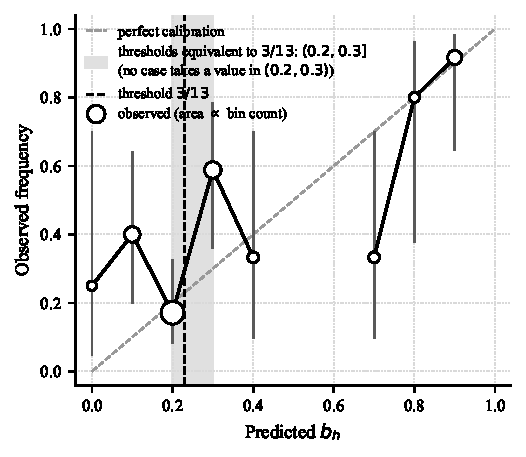
\includegraphics[width=\columnwidth]{reliability-needs-human.pdf}
    \caption{Reliability of the \texttt{needs\_human} marginal over all 100 cases,
    ECE 0.142 (bootstrap 95\% CI $[0.100, 0.249]$, median 0.171). Points above the
    diagonal are under-confident: the belief reports a low probability where the
    observed frequency is high. Marker area is proportional to bin count and bars
    are Wilson 95\% intervals, because the bins hold between 4 and 35 cases and
    most are individually consistent with perfect calibration. The vertical line is
    $b_h^{\star} = 3/13 \approx 0.231$; the shaded band is the interval of
    thresholds that decide identically, which is the half-open $(0.2, 0.3]$. The
    two brackets are not interchangeable: the elicited marginal takes only
    one-decimal values, so no case falls in the \emph{open} interval $(0.2, 0.3)$,
    while 17 of the 100 cases sit at exactly $0.3$ and a threshold placed there
    still puts all 17 on the escalate side. The bin that
    \emph{contains} the threshold, 0.2--0.3, is the largest ($n = 35$) and is very
    slightly over-confident (predicted 0.200, observed 0.171, CI $[0.081, 0.327]$).
    Its neighbours at 0.1--0.2 and 0.3--0.4 are under-confident by 0.300 and 0.288.
    The 0.7--0.8 bin reads over-confident by 0.367 on 6 cases, but its interval
    $[0.097, 0.700]$ covers the predicted value, so the belief is not uniformly
    under-confident and that bin is not evidence of the reverse. Bins 0.5--0.7 are
    empty, hence the break in the curve.}
    \label{fig:reliability}
    \end{figure}
    
Every one of the 16 missed escalations in the 100-case run of
Table~\ref{tab:results} came from the same place: the belief
under-estimated the needs-human probability, not the readiness. On all 16, the
needs-human estimate was 0.30 or below against a true label of needing a human,
while the readiness argmax on those same cases was spread across cold, hot, and
warm and was often correct and confident. The belief reads under-confident on the
needs-human marginal, with an expected calibration error of 0.142 (bootstrap 95\%
CI $[0.100, 0.249]$; 0.168 on the development half, 0.184 on test), and reliability
bins (Figure~\ref{fig:reliability}) that read low against observed frequency near
the escalation threshold (for example, a predicted 0.10 against an observed 0.40,
and a predicted 0.30 against an observed 0.588).

Two qualifications belong with that number. First, the bin that actually
\emph{contains} $3/13$ is not the under-confident one: at 0.2--0.3, the largest bin
at $n = 35$, predicted 0.200 against observed 0.171, the belief is very slightly
\emph{over}-confident, and its Wilson interval $[0.081, 0.327]$ covers the
predicted value. The under-confidence is in the neighbouring bins. So
``under-confident exactly where the threshold sits'' is not the right description;
the mechanism is that a large mass of cases sits pinned at $b_h = 0.20$, just below
the line, and 35\% of the case set turns on whether that single elicited value is
right. Second, with 4 to 35 cases per bin most individual bins are consistent with
perfect calibration, so the ECE point estimate carries most of the evidential
weight here and its interval is wide.

Because the failures trace to the needs-human marginal rather than to the readiness
marginal, recalibrating that marginal is the natural first fix. Two fits are
reported and they are not interchangeable: Section~\ref{sec:failure} fits on all
100 cases and is an in-sample ceiling, while the fit below is fitted on 50
development cases and scored on the 50 test cases. This is weaker than the claim
an earlier draft made. That the misses localise to one marginal is consistent with
the independent two-part belief, but it is not evidence \emph{for} independence: the
experiment records only the two marginals, never the joint, so it cannot detect the
two components interfering even if they did. Testing independence would require
eliciting $P(s, h)$ directly and comparing it against $P(s)\,P(h)$, which this run
does not do.

\paragraph{A finer belief, fitted on one half and scored on the other.}
The diagnosis above is a claim about the elicitation, so it can be tested by
changing the elicitation. Re-eliciting $b_h$ as an expectation over the model's
digit logprobs, rather than as a probability the model writes out in words,
replaces the eight one-decimal values it produced over the 100 cases with 43
distinct scores on the 50 test cases. The elicitor itself was chosen on the
development half by cross-entropy: reading the digit distribution reaches 0.9934
bits there against 1.8004 bits for asking the model Yes or No and taking the
probability of Yes, a margin of 0.8071 bits. Three candidate maps were then fitted
on those same 50 development cases --- identity, Platt, isotonic --- under a rule
fixed before the fit, that an order-preserving map is kept unless a merging one
beats it by more than 0.02 bits. Isotonic reached 0.8356 bits against Platt's
0.9103 and identity's 0.9934, a margin of 0.0747, so the merging map was taken and
the shipped map does not preserve the ranking of the test scores. Applied unchanged
to the 50 test cases, it improves all three proper scoring rules named in advance:
cross-entropy 0.8546 to 0.8136 bits, against a label entropy of 0.9815 bits at a
base rate of 0.42; ECE 0.1526 to 0.0696; Brier 0.2063 to 0.1962, with the 43
distinct scores merged to 33. On those same 50 cases the policy driven by the
calibrated score stops using \emph{answer} at all: its action census goes from
\{\emph{answer} 12, \emph{escalate-notify} 21, \emph{hold} 17\} to
\{\emph{escalate-notify} 41, \emph{hold} 9\}, so on this arm the two never-used
actions of Section~\ref{sec:unused} are three. The trade-off is sharpest in the
escalation rates on those 50 cases: precision falls from 0.667 to 0.463 while
recall rises from 0.667 to 0.905, so the calibrated belief catches nearly every
case that needs a human and pays for it by escalating most of the ones that do
not. These are not two findings. The
second is caused by the first, and the cause is the map's range rather than the
scores it happened to produce.

\paragraph{Why \emph{answer} disappears.}
Isotonic regression by PAVA sets each pooled block's level to that block's own
positive rate. The lowest block of the committed map pools 23 of the 50 development
cases, 6 of which are positive, so its level is the probability
$6/23 = 0.260870$ --- the reachable-score floor of the map, a probability and not a
count --- and no input can make the map emit a score below it. The interval
$[0, 6/23)$ is unreachable rather than merely unpopulated. The boundary the score
has to fall below for \emph{answer} to be the cheapest action is
$b_h^{\star} = 3/13 \approx 0.230769$, and it lies inside that unreachable
interval:
\begin{equation}
\frac{1}{5} < \frac{3}{13} < \frac{6}{23} ,
\end{equation}
an ordering that spans less than 0.061 end to end, which is why all three are
carried as exact rationals rather than to two decimal places. Of the 50 test
cases, 24 sit below $3/13$ on the raw score and none does after the map. The
calibrated arm is therefore a two-action policy by construction rather than by
preference, and the same ordering settles the constrained-menu region of
Section~\ref{sec:unused}, since $6/23$ is above the $1/5$ bound as well. This is a
statement about the map's range and not about how many cases land on it: of the 100
scored cases exactly one sits at the reachable-score floor, and it is a development
case, because interpolation lifts the rest of the lowest block strictly above it.
The transferable form is that a PAVA-fitted
map's reachable range is bounded below by the positive rate of its lowest pooled
block, and that cross-entropy, ECE and Brier never check whether a policy's fixed
thresholds sit inside that range.

\begin{table}[t]
\centering
\begin{tabular}{lrrr}
\toprule
Arm, on the 50 test cases & Total & Mean & Miss \\
\midrule
re-elicited, uncalibrated & 70 & 1.40 & 7 \\
re-elicited, calibrated   & 75 & 1.50 & 2 \\
written belief            & 86 & 1.72 & 8 \\
always-notify             & 87 & 1.74 & 0 \\
\bottomrule
\end{tabular}
\caption{Secondary numbers for the held-out fit, on the 50 test cases only. Total
is the realised cost over those 50, Mean is per case, and Miss is missed
escalations out of 50. These are reported next to the calibration metrics and are
not the claim; the claim is the three proper scoring rules. The test half carries
only 8 of the 16 missed escalations of the full 100-case run
(Table~\ref{tab:results}), so a change of one or two misses on this half is not
evidence. The written-belief row re-elicits the one-decimal probability of that run
and reaches the same total, mean and miss count on this half as its cached beliefs
do --- aggregate agreement only, not a case-for-case replay. It also shows why the
denominators matter: the mean is unchanged from the 100-case run at 1.72 while the
miss count is half, so the mean may be compared across the two populations and the
count may not. The two re-elicited rows are the calibration contrast, 7 misses of
50 down to 2 of 50 at a mean rising from 1.40 to 1.50 --- breakable, and not free.
Always-notify escalates all 50 by construction and the calibrated arm escalates 41
of them, so much of what calibration buys here is a move toward blanket
escalation.}
\label{tab:calibration}
\end{table}

\paragraph{What the held-out fit does and does not settle.}
Table~\ref{tab:calibration} carries the cost and miss numbers for four arms on the
test half, and they are secondary: the claim is the three scores above. The fit
itself is a fit on one half of a synthetic set scored on the other, and
Section~\ref{sec:split} has already said that the two halves are matched by
construction, so it is not evidence that the belief would transfer to a deployment.
What it is evidence for is narrower: the improvement in the three scores does not
come from fitting the cases it is scored on. The two operations on the population
also have to be kept apart. Section~\ref{sec:failure} fits the marginal on all 100
cases in-sample and halves the misses from 16 to 8; restricting the same policy and
the same beliefs from those 100 cases to these 50 also produces 16 to 8, and the
two have nothing in common beyond the pair of numbers. Every miss count in this
subsection carries the case set it was counted on for that reason.

\section{Failure analysis}
\label{sec:failure}

The cost-aware policy makes 16 missed escalations and no other class of error
worth naming: no hard-constraint violations, and its needless actions are the
cheap ones the design is willing to pay. So the failure analysis is almost
entirely about the misses. Five are examined in detail below, chosen to cover the
distinct ways a miss happens.

\subsection{The shared cause}
All 16 misses have the single cause described in Section~\ref{sec:results}: an
under-estimated needs-human probability. None of them come from the two hidden
components being confused with each other. This matters for how the misses should
be counted. Treating every miss as a false assertion at cost 10 overstates the
damage, because a \emph{hold} is a partial hedge: it is the wrong action, but it
does not deliver a false answer, so the matrix charges it 3 or 4 rather than 10.
Across the 16 misses the realised costs are nine at 10, four at 3, and three at 4,
for 114 in total, not the 160 that costing every miss at 10 would give.
One caveat belongs with this diagnosis. That every miss traces to an
under-estimated needs-human probability is a statement about this labelling
scheme, not a proof of the underlying causal mechanism: the experiment does not
independently exclude cost-model misspecification, the coarse three-state
readiness space, or the one-decimal quantization of the belief as contributing
causes, and the recalibration in §7.3 is an in-sample ceiling rather than a
held-out test.
\subsection{Five cases}
Table~\ref{tab:failures} lists five misses and the mode each one represents.

\begin{table}[t]
\centering
\begin{tabular}{lr p{3.2cm}}
\toprule
Case & Cost & Mode \\
\midrule
a11-repeated-097 & 10 & tie-break, not the cost model; since corrected \\
a04-booking-042 & 10 & readiness right, needs-human wrong \\
a02-deep-015 & 10 & one quantization step below the line \\
a03-followup-024 & 4 & hold looked cheap, readiness also off \\
a10-persistent-091 & 3 & cheapest miss the matrix allows \\
\bottomrule
\end{tabular}
\caption{Five missed escalations, one per failure mode. All five are from the
reported run. The first has since been fixed in the implementation and is retained
because the reported run predates the fix; the other four remain open.}
\label{tab:failures}
\end{table}

The three that realise the full cost of 10 fail in different ways.
\texttt{a04-booking-042} is the cleanest illustration of the shared cause: the
readiness estimate was right and confident, and only the needs-human number
failed, so nothing about readiness could have saved it. \texttt{a02-deep-015} sits
one quantization step below the line: its elicited $b_h$ is 0.20 against a threshold
of 0.2308. Describing this as missing by 0.031, as an earlier draft did, reads the
gap as a small numerical shortfall, which overstates how close the call was. The
belief cannot express 0.24; the next value it can emit is 0.30. Recovering this case
requires moving it a full decimal step, not nudging it by three hundredths, and the
same is true of the 35 cases that share its $b_h = 0.20$. \texttt{a11-repeated-097}
is the worst of the three, for a reason that is not the cost number --- and, unlike
the other four cases in Table~\ref{tab:failures}, it is not an open failure: its
cause was identified and repaired, and it is retained here because the reported run
predates the repair. Its belief is the furthest from the flip point of any miss: it
needed a needs-human estimate above 0.50 and the model reported 0.00, so
recalibration would not save it the way it would save the near-threshold cases. And
it was not decided by the cost model at all. Two actions came out with an expected
cost of exactly 0.000, and the tie was broken by the fixed ordering of the action
list rather than by any cost comparison. In the true state, holding would have cost
3, so 7 of its 10 realised points were attributable to an implementation detail, the
tie-break, rather than to a property of the policy.

That detail has since been repaired, as Section~\ref{sec:method} notes. Ties now
resolve safest-first, in an order derived from the cost matrix by worst-case cost
(\texttt{tie\_break\_order}) rather than hand-written, which gives
\emph{escalate-notify} (worst case 3) $<$ \emph{ask} (4) $<$
\emph{escalate-pause} (6) $<$ \emph{hold} (8) $<$ \emph{answer} (10). The old
ordering resolved indifference toward \emph{answer}, the action with the largest
downside, which is the opposite of what a policy premised on the expense of false
assertion should do. Exactly one decision on the reported case set changes:
\texttt{a11-repeated-097} moves from \emph{answer} to \emph{hold}, and the mean cost
falls from 1.720 to 1.650 --- the 7 points this section predicted, and no others.
Miss count and escalation count are unchanged at 16 and 43, since \emph{hold} and
\emph{answer} are both non-escalating actions. This is also the only decision the
correction \emph{could} change: \texttt{a11-repeated-097} is the one case in the 100
where two feasible actions come out at exactly equal expected cost, and a tie-break
is consulted nowhere else. The uniform baseline is unaffected, for a structural
reason worth stating --- with every non-zero cost set to one, all five actions have
worst-case cost 1, so the derived order degenerates to the declaration order and the
baseline's 2.58 is identical under both rules. Table~\ref{tab:results}
reports the pre-fix numbers, because \texttt{results/run.json} was generated before
the change and is kept as the artifact the reported numbers are checked against;
\texttt{run\_policies.py -}\texttt{-legacy-tie-break} reproduces it exactly, action
for action on all 100 cases, so those numbers stay verifiable while the default path
uses the corrected rule.

The two cheaper misses show why not every miss is a false assertion.
\texttt{a03-followup-024} and \texttt{a10-persistent-091} were held rather than
answered, so they cost 4 and 3 rather than 10. For these the binding comparison
is hold against escalate-notify, not answer against escalate-notify, and because
the hold row is not flat across readiness their thresholds are readiness-dependent
rather than the clean 3/13 of the answer cases. Reporting them at their true cost,
rather than rounding every miss up to 10, is what keeps the miss total honest.

\subsection{What recalibration actually recovers}
Since the diagnosis above points at the needs-human marginal, it can be tested
directly rather than left as a prediction. Replacing each elicited $b_h$ with the
observed frequency of its reliability bin --- histogram binning, fit on the same
100 cases, so this is an optimistic in-sample ceiling and not a held-out result ---
and re-running the policy gives mean cost 1.250 against the corrected baseline of
1.650, and 8 misses against
16.

The composition of that change matters more than the totals. Of the 16 original
misses, 9 are fixed and 7 survive. The survivors are the cases the diagnosis
already flagged as out of reach: 6 sit at $b_h = 0.20$, in the bin whose observed
frequency (0.171) is itself below the threshold, so recalibration moves them the
wrong way, and 1 is \texttt{a11-repeated-097} at $b_h = 0.00$. Recalibration also
\emph{creates} one new miss: \texttt{a06-frustrated-055}, at $b_h = 0.70$, is pulled
down into the over-confident 0.7--0.8 bin and switches from
\emph{escalate-notify} to \emph{hold}.

The cost is paid in human load. Escalations rise from 43 to 60, precision falls from
0.605 to 0.567, and recall rises from 0.619 to 0.810. Recalibration does not make
the policy better on every axis; it buys recall with load, and 8 misses remain that
no amount of recalibrating this marginal removes. That residual-miss floor, not the
halving, is the finding.


\subsection{A failure the test set cannot show}
One failure did not come from the synthetic run at all. In a live deployment a
lead sent a routine request for information and, before the agent had replied, a
second short message asking to be contacted directly by a person. The agent acted
on the routine message and silently dropped the second, which carried the only
needs-human signal in the turn. The rare, high-cost signal was averaged away by
the common, low-cost one because the two messages were handled as a single turn.

This is a different kind of failure from the 16 misses. Those are belief-scoring
errors on a single message. This one is a turn-boundary error: the important
message never received its own belief evaluation. The synthetic test set cannot
produce it by construction, because every case carries one message as a single
string and the harness scores one message per turn. Surfacing this class of
failure would need multi-message-per-turn cases and a per-message evaluation step
before the turn is acted on, neither of which this experiment has, so none of the
numbers reported here bear on it. It is recorded here, and as a limitation in
Section~\ref{sec:limitations}, rather than left out because the harness happens
not to reach it. It is also the failure that several practitioners, on being shown
it, independently proposed the same fix for: scan each message for a small set of
critical intents before the turn is scored as a whole, so that a rare handoff
signal overrides rather than averages into the turn.
\section{Limitations, ethics, and human control}
\label{sec:limitations}

\subsection{Limitations}
The results rest on synthetic data, and several of the paper's numbers are only
measurable because of that. The clearest case is recall on missed escalations. In
a live inbox there is no label for the lead who needed a human and did not get
one, so escalation recall cannot be measured at all; it is measurable here only
because the cases are labeled by construction. The needs-human base rate of 42\%
was chosen so that recall is estimable. Earlier drafts described it as inflated
above a real inbox; that comparison is withdrawn, because no measured base rate for
this channel exists to compare against. What can be said without a source is
narrower and still sufficient: the rate was set for measurability rather than
sampled, so the precision and recall reported here are properties of this case set
and should not be expected to transfer to production, in either direction. The
readiness distribution is off the design's own prior in the same way: the belief
module assumes 85\% cold, the case set is 39\% cold.
The readiness and needs-human labels are the author's
judgment of what each message was written to represent, not outcomes observed from
real leads, so they carry the author's assumptions about intent.

Two scope limits on the headline result belong here as well as in
Section~\ref{sec:results}. The cost improvement is against the uniform baseline
only: against always-notify the comparison is a near-tie, 1.72 against 1.74, so the
cost-aware policy is not the cheaper policy and is not claimed to be. What it buys
is human load --- it escalates 43 times out of 100 rather than all 100, at a
precision of 0.605 against 0.420 --- and that operational reduction, not a cost
win, is the claim. The second is the development and test split. Both halves reach
the same total cost, but the split was stratified by archetype and sub-variant and
balanced on the needs-human count, so the halves are matched by construction and
the agreement follows from that; it is not out-of-sample evidence and is not read
as any.

The state space is deliberately coarse and this costs the model in two visible
ways. Non-leads such as competitors and abusive messages are labelled cold rather
than given their own state, which slightly distorts readiness calibration. And the
state cannot separate a competitor fishing for pricing from an abusive message:
both come out as cold and needing a human, yet the two call for different actions.
The state space simply cannot see the difference, which is a real finding about
its granularity rather than a bug in the policy.

Several limitations are structural to the method rather than to the data, and the
first is one an earlier draft got backwards. The policy is myopic: it minimises
immediate expected cost and carries no machinery that prices the better belief a
question buys on the next turn. That much is a true statement about the
implementation and stays a limitation of it. What does not survive is the
inference drawn from it --- that the \emph{ask} action is therefore undervalued
here, that the honest handling this design omits would be to compute its value of
information, and that \emph{ask}'s absence from the results follows from the
horizon. Section~\ref{sec:unused} computes it. On the unconstrained action menu
the value of one more question is at most $-2/13$ at every belief
(Theorem~\ref{thm:ceiling}); posteriors are beliefs, so the bound binds at every
node of a lookahead tree and the budgeted family collapses, $W_k =
V_{\mathrm{act}}$ for every $k \ge 1$. Asking is not underpriced by the one-step
rule. It is priced, and it loses at every depth. That is a withdrawal rather than
a qualification, because the claim asserted a direction the analysis reverses.

What remains is narrower, and it belongs here rather than in the results. The
collapse is a property of this cost matrix, and the policy never checks the
property it depends on. A question can be rational on the unconstrained menu only
where $c_F/\nu + c_T/\alpha < 1$; this matrix gives $16/15$, and scaling the
\emph{ask} row by $15/16$ would put the ceiling exactly at zero. On a matrix that
satisfied the condition, lookahead would be worth having and this design would
have nothing with which to take it --- there, being myopic would cost what the
earlier draft said it costs here. So the statement that survives is not that
asking is mispriced but that being myopic is safe on this matrix, for a reason the
policy does not verify. Two readings are wrong and worth naming: $2/13$ is a floor
on the gap and not an estimate of its size, and the theorem bounds one more
question inside a deeper policy on this matrix and this action menu, not the value
of interaction design in general. Where a question can pay is the constrained
menu, at $b_h < 1/5$ on the hot ray, and Section~\ref{sec:unused} shows that
region is empty here --- structurally so on the calibrated beliefs, whose
reachable range starts above $1/5$, and contingently on the published ones.

The value-of-information analysis carries a boundary of its own, and it is worth
saying exactly where it falls. Computing the continuation term needs an answer
model: a distribution $P_b(u)$ over what the lead would reply and a posterior
$b^u$ for each reply. Both are simulated from the design's own model of the lead,
the same one that produced the belief being scored, so a check that the
computation agrees with its own definitions is a self-consistency check of the
implementation. It is not evidence that the answer model matches how real leads
reply, and nothing here measures that: a second turn per case would be new data.
What that bounds is narrow, and the narrowness is the point.
Theorem~\ref{thm:ceiling} does not use the answer model at all --- it needs only
that the continuation term is non-negative, which follows from
Table~\ref{tab:costs} alone. The quantities that do depend on the answer model are
the per-case ceilings and the count of questions that resolve the state, not the
result that \emph{ask} is never selected. What is unvalidated is the model of the
reply; what does not rest on it is the bound.

Abstention is priced out under this matrix, and that is a bounded result rather
than an option left untested. \emph{Escalate-pause} is dominated by
\emph{escalate-notify} in every one of the six columns of Table~\ref{tab:costs},
by between 1 and 3, so a rule that hands the conversation over instead of
notifying raises realised cost on every case it touches and cannot lower the count
of missed escalations at all (Section~\ref{sec:unused}). With \emph{ask}
unselected as well, the reported results exercise three of the five actions. The
scope of that is the matrix, not the design space. These costs are expert-set
rather than measured, and Section~\ref{sec:model} shows at least one magnitude is
load-bearing, so a matrix in which pausing is not dominated --- one that prices an
unattended conversation, or a handover acted on sooner than a notification ---
would make abstention available again, and this experiment says nothing about that
case. What it settles is that abstention does not help under these costs, not that
it never helps. And the hard constraint that removes
the answer action on restricted cases is treated here as observable and
error-free, because a flag on the case says the message asks for legal or land
documents. A production detector for that condition
would carry its own false-positive and false-negative rates, which this experiment
does not model. Sweeping a synthetic false-negative rate on that flag from 0 to 0.5
changes nothing --- cost stays at 1.650 and misses at 16 --- but that is not
reassurance, it is a restatement of the fact that the constraint never bound: on all
8 restricted cases the policy already escalates on cost grounds, so dropping the flag
changes no decision. A detector's error rates would matter on restricted cases the
cost model does \emph{not} already catch, and this case set contains none.

A further structural limitation is the granularity of the belief itself. The
elicited $b_h$ takes only 8 distinct values across the 100 cases, every one at a
single decimal place, distributed
$\{0.0{:}\,4,\ 0.1{:}\,15,\ 0.2{:}\,35,\ 0.3{:}\,17,\
0.4{:}\,6,\ 0.7{:}\,6,\ 0.8{:}\,5,\ 0.9{:}\,12\}$. The language model is being asked
for a probability and is returning something closer to an ordinal grade. Three
consequences follow, and all three are visible in the results: the threshold $3/13$
cannot be distinguished from any other value in $(0.2, 0.3]$; 35\% of the case set
rests on one elicited value, $b_h = 0.20$, sitting just below the line; and
recalibration cannot rescue those 35 cases, because it maps a bin to a single
number and that number (0.171) is also below the line. A finer-grained elicitation
is the prerequisite for most of the improvements this paper proposes, and it is not
tested here. Relatedly, the beliefs come from a single unpinned model
(\texttt{gpt-4o-mini}) elicited once per case; no dated snapshot is recorded, no
repeat elicitation measures the variance of the belief itself, and every number in
the paper is conditional on that one draw. A re-elicitation at temperature 0
returns the same belief for 89 of the 100 cases and a different one for 11, with
none unparseable. What the record contains does not determine the cause, and the
count is reported here rather than explained.

Reproducibility has a boundary inside the artifact and another outside it. Inside:
every number reported here is regenerated from the committed beliefs by the
committed code, deterministically, and the data artifacts are compared byte for
byte --- except two that carry floats whose exactness depends on the interpreter,
because compensated summation over floats arrived in CPython 3.12. That version is
declared as the floor, and those two files are compared to a tolerance of
$10^{-9}$ rather than exactly. The rendered figure is excluded from the byte
comparison outright: a PDF records the version of the renderer that drew it and the
moment it was drawn, so its bytes move when neither the data nor the code has.
Every value the figure plots is checked against the run artifact instead, which
verifies the numbers and not the drawing. Outside: the beliefs are not reproducible
from scratch, for the reason just given, so the committed cache is an input to the
experiment rather than an output of it, and regenerating it would move every number
in this paper.

Because the case set's readiness distribution does not match the prior the design
assumes, the reported means are sensitive to reweighting. Importance-weighting each
case toward the module's own prior (weights: hot 0.087, warm 0.342, cold 2.180)
moves the cost-aware policy from 1.720 to 1.456 and the uniform baseline from 2.580
to 2.526 --- the gap widens from 0.86 to 1.07. It also reverses the comparison
against always-notify, which moves from 1.740 to 1.834. The direction of the main
result survives reweighting; its magnitude does not. Since the prior itself is
expert-set rather than measured, neither weighting is the authoritative one, and the
spread between them is the honest statement of what the case set can support.

Finally, one whole class of failure is invisible to the test set by construction.
As Section~\ref{sec:failure} describes, a high-cost signal batched with a routine
message at a turn boundary cannot occur in a set where every case is a single
message scored on its own. This is the sharpest version of the general point that
synthetic data trades realism for measurability: here the trade hides not a
distorted number but an entire failure mode.

\subsection{Ethics and human control}
The system decides when a person is pulled into a conversation, and the costs are
set to make missing a needed human more expensive than a needless handoff. That is
deliberate, but it means the agent will sometimes escalate cases that did not need
it, spending human attention as the price of not missing the ones that did. The
hard constraint on false legal and land claims is the other side of this: some
answers are treated as a line the agent may not cross at any belief, rather than a
cost to be traded off, because the harm of a confident false claim on a
consequential matter is not the kind of thing a cheaper action elsewhere should be
able to outweigh.
The experiment only measures the cost of choosing to escalate. It doesn’t account for what happens afterward—such as human mistakes, limited capacity, or unclear accountability. Those are left for future research.
A deeper point raised in the live discussion is worth recording as a direction the
current design does not yet meet. The turn-boundary failure is not only a scanning
problem; the underlying issue is that a message was droppable at all. A more robust
design would make every inbound item durable, with an explicit acknowledge or
close step, so that a request for a human keeps returning until something resolves
it, regardless of how a later ranking scores its priority. Priority can be fuzzy;
existence should not be. The present design scans for critical signals before the
turn is acted on, which reduces the risk, but it does not yet guarantee that no
message can be silently dropped, and that guarantee is the right target for a
production system.

\section{Conclusion and new questions}
\label{sec:conclusion}

This paper built a small agent that decides, on each inbound message, whether to
answer, ask, hold, or escalate to a human in one of two ways, when the lead's
readiness and whether they need a person are both hidden. The decision rule is a
textbook one: minimise expected cost under a belief. The contribution is not the
rule but an honest account of what it buys. Making the cost matrix asymmetric
cuts mean cost by a third against the same rule without that asymmetry. Against a
policy that simply escalates everything, it does not cut cost at all, and the
paper says so; what it buys there is reaching the same cost while escalating fewer
than half as often. Every missed escalation traces to the needs-human marginal
rather than to the readiness marginal, which points at recalibration rather than
redesign --- though, as Section~\ref{sec:results} notes, that localisation is
consistent with the two-part belief without being evidence for it, since the
experiment never observes the joint distribution.

Three questions follow directly from these results. This version closes one of them,
answers most of another, and leaves the third open.

The first is calibration, and it is the one it answers most of. Recalibrating the
needs-human marginal in-sample halves the misses on those 100 cases, from 16 to 8,
and cuts mean cost from 1.650 to 1.250 --- but the composition is 9 fixed, 7
surviving, and 1 newly created, and escalations rise from 43 of 100 to 60 to pay for
it. The residual-miss floor is real and it has a specific cause: 6 of the 7
survivors sit at $b_h = 0.20$, in a bin whose observed frequency is also below the
threshold, so no mapping of that bin to a single value can rescue them. It is
therefore set by the granularity of the elicitation, not by the calibration method
--- and that last claim is the one thing here that can now be reported as tested
rather than asserted. What an earlier draft named as the next step, a finer-grained
belief and a held-out recalibration fit, is Section~\ref{sec:calibration}: eliciting
$b_h$ from digit logprobs and fitting the map on 50 development cases takes the
misses on the other 50 from 7 of 50 to 2 of 50. That residual-miss floor was
breakable, and it broke when the elicitation got finer, which is what the claim
predicted. It was not free. The mean rises from 1.40 to 1.50 on that half and the
calibrated arm escalates 41 of the 50, because a PAVA-fitted map cannot emit a score
below the positive rate of its lowest pooled block and the threshold for answering
lies underneath that reachable-score floor. So the granularity claim survives and
the bound moves: out of the elicitation, into the calibration map.

The second is the ask action, and it is the one that closes. An earlier draft left
it open as a question --- whether asking is genuinely useful or merely unpriced ---
and the answer is neither. It is priced, and it loses. Scoring the action by its
one-step value of information is what Section~\ref{sec:unused} does, and what comes
out is a bound rather than a measurement: on the unconstrained action menu the value
of one more question is at most $-2/13$ at every belief in the simplex
(Theorem~\ref{thm:ceiling}), attained at the all-hot vertex, so there is no belief a
deployment could reach at which the question is worth its fee. Nor is that an
artefact of the one-step horizon. Posteriors are beliefs, so the same bound holds at
every node of a lookahead tree, and the budgeted family collapses:
$W_k = V_{\mathrm{act}}$ for every $k \ge 1$. Asking does not fail here because the
policy looks only one step ahead. It fails at every depth. \emph{Ask} is selected
zero times out of 100 and \emph{escalate-pause} zero times as well, and the
five-action set is a three-action set in practice --- what this version adds is that
the two zeros follow from the cost matrix rather than from the case set.

What transfers is not that number but the condition behind it. A question can be
rational at some belief on the unconstrained menu only if
$c_F/\nu + c_T/\alpha < 1$: the fee for asking when no human is needed, measured
against the cost of a needless escalation, plus the fee for asking when one is,
measured against the cost of a false answer, together coming to less than the whole.
Here they come to $16/15$, so the condition fails, and it fails by 6.25\% ---
scaling the \emph{ask} row by $15/16$ puts the ceiling exactly at zero. A designer
with a cheaper question, a single tap or an inference from metadata already
collected, is on the other side of that line, and the same inequality says where the
line is. Asking
is not useless in general. On this matrix, and on the unconstrained menu, it is
priced out; Section~\ref{sec:unused} also carves out the one place it is not, where
the hard constraint removes \emph{answer} and the ceiling turns positive over a
region of hot beliefs that no case in this set occupies.

The third is the turn boundary. The one failure the synthetic test set cannot
produce is the one that came from a live run, where a high-cost signal was lost
when batched with a routine message. Building cases with more than one message per
turn, and a per-message scan that lets a rare critical signal override the turn,
would let this failure be measured rather than only reported, and would test the
durability idea that no inbound message should be silently droppable in the first
place.
% --- References (required block 12) ---------------------------------------
% The kit's two bibliography commands. named.bst sits next to this file and
% generates its own "References" heading, so there is no \section* here.
% Switched on because references.bib now has entries and the paper cites five
% of them; see the citation-macro note in the preamble before adding more.
\section*{AI-use statement}

This project was built with AI assistance used as a tool under the author's
direction, not as an author. The author selected the problem, made and locked
every design decision, set the cost values and their ordering, wrote all public
discussion contributions personally, and verified every reported number against
the committed run artifacts.

AI tools were used for: preparing research terms, search queries, and candidate
communities and accounts to engage [tools:\ Claude, ChatGPT, Gemini]; studying the
source papers [tool:\ NotebookLM]; scaffolding, writing, and repairing code,
running the test harness, and executing commits [Claude and Claude Code]; and
adversarial review passes of the draft [tools used, logged in
\texttt{review-record.md}]. Per-decision provenance --- what the author set
versus what a tool proposed --- is recorded at the point each decision was made
in \texttt{build-log.md}.

Every AI output was checked before use. Where a tool was confidently wrong, the
error and its correction are recorded rather than propagated; these are logged in
the ``Important AI errors'' section of \texttt{research-file.md}. Two are worth
naming: a synthesis that recommended an architecture directly contradicting the
locked design, and an unverified bound attributed to a mis-cited source, neither
of which was carried into this paper.

The author affirms that no conversation in the discussion record is fabricated;
that every reported result comes from a real run of the committed code over the
committed data; and that no reference is cited that the author did not read.
\bibliographystyle{named}
\bibliography{references}

\end{document}
